\documentclass{article}
\usepackage{graphicx}
\usepackage{algorithm}
\usepackage[noend]{algorithmic}
\usepackage{subfigure}
\usepackage{amssymb, amsmath, graphicx, charter, latexsym}
\usepackage{layouts}
\usepackage[letterpaper]{geometry}
\usepackage{enumerate}
\usepackage{epstopdf}
\usepackage{ragged2e}
%\usepackage{times}
\usepackage{mathtools}
%\usepackage[scaled]{helvet}
\usepackage{mathptmx}
\usepackage{verbatim}
\usepackage{listings}
\usepackage{siunitx}

\lstset{
basicstyle=\ttfamily,
}

\begin{document}

\title{\bf ECEN 689-- Real-Time Wireless Networks: Project 2\\ (Due on 4/1)}
\date{}
\author{%
Ping-Chun Hsieh\\
\texttt{lleyfede@tamu.edu}
\and
Tao Zhao\\
\texttt{alick@tamu.edu}
\and
Dongni Han\\
\texttt{handongni2015@tamu.edu}
}
\maketitle

\section*{Terminology}

In our report, we use ``server'' to denote the WiFi access point (AP), and
``client'' to denote the terminal device such as a mobile phone, a tablet, and
so on. Throughout our simulation, we let node $0$ be the server, and node $1$ be
the client, which correspond to the device A and B in the problem descriptions
respectively.

S-WiFi is the name of our application as well as our project. It stands for
Smart WiFi, or whatever you think it is.

\section*{Simulation Setup}
\begin{table}[htbp]
\centering
    \caption{Parameters of the wireless channel.}
    \vspace{2mm}
    \begin{tabular}{ | l | l | }
    \hline
    Item & Value \\ \hline
    Path loss exponent & 2.0  \\ \hline
    Shadowing deviation & \SI{4.0}{dB} \\ \hline
    Reference distance & \SI{1.0}{m} \\
    \hline
\end{tabular}
\label{table: channel}
\end{table}
Throughout the report, we consider a single wireless link between two devices, say A and B. The transmitter power level is \SI{10}{mW}. We use the shadowing module as the wireless channel. The parameters of the channel are summarized in Table \ref{table: channel}.

\begin{table}[htbp]
\centering
\caption{Parameters of the 802.11b MAC.}
    \vspace{2mm}
    \begin{tabular}{ | l | l | }
    \hline
    Item & Value \\ \hline
    Data rate & \SI{11}{Mb/s}  \\ \hline
    Basic rate & \SI{1}{Mb/s}  \\ \hline
    PLCP data rate & \SI{1}{Mb/s}  \\ \hline 
    Preamble length & \SI{144}{bits} \\ \hline
    Slot time & \SI{20}{\mu s} \\ \hline
    SIFS & \SI{10}{\mu s} \\
    \hline
\end{tabular}
\label{table: mac}
\end{table}

For the medium access control (MAC) layer, we use the 802.11 module built in ns-2. Following the IEEE 802.11b standard, the MAC layer parameters are chosen as in Table \ref{table: mac}.


\section*{Uplink Transmissions with PCF}
\label{section: uplink}



\section{Baseline Policy}
\label{section: baseline}


\section{Implementation in NS-2}
\label{section: ns2}


\section{Simulation Results}
\label{section: simulation}
\subsection{Symmetric System with 2 Clients}
Real-time and non-real-time traffic
\subsection{Asymmetric System with 2 Clients}

\subsection{System with N Clients}
%\begin{figure}[htbp]
%\centering
%\subfigure[Downlink round-trip time.]{
%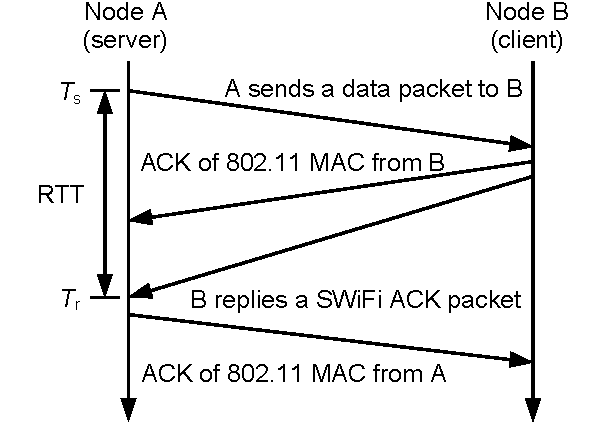
\includegraphics[scale = 0.7]{downlink_rtt.pdf}}
%\subfigure[Uplink round-trip time.]{
%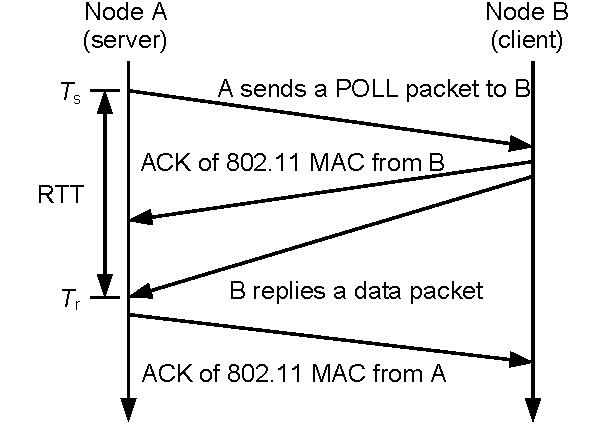
\includegraphics[scale = 0.7]{uplink_rtt.pdf}}
%\caption{Round-trip time when node A and node B are close to each other.}
%\label{figure: rtt}
%\end{figure}


\end{document}
